\documentclass{article}

\usepackage{neurips_2026}

\usepackage[utf8]{inputenc}
% Note: [T1]{fontenc} omitted — tectonic/XeLaTeX uses Unicode natively;
% T1 + amsfonts + LM Typewriter triggers a "Missing $" crash in XeLaTeX.
\usepackage{hyperref}
\usepackage{url}
\usepackage{booktabs}
\usepackage{amsfonts}
\usepackage{amsmath}
\usepackage{nicefrac}
\usepackage{microtype}
\usepackage{xcolor}
\usepackage{graphicx}
\usepackage{tikz}
\usepackage{pgfplots}
\usepackage{pgfplotstable}
\usepackage{multirow}
\usepackage{array}

\usetikzlibrary{arrows.meta, positioning, shapes.geometric, fit,
                backgrounds, decorations.pathreplacing, calc}
\pgfplotsset{compat=1.18}

% ── colour palette ────────────────────────────────────────────────
\definecolor{nodeblue}{HTML}{1565C0}
\definecolor{nodepurple}{HTML}{6A1B9A}
\definecolor{nodegreen}{HTML}{2E7D32}
\definecolor{nodeorange}{HTML}{E65100}
\definecolor{nodeteal}{HTML}{00695C}
\definecolor{nodegray}{HTML}{424242}
\definecolor{lightblue}{HTML}{E3F2FD}
\definecolor{lightpurple}{HTML}{F3E5F5}
\definecolor{lightgreen}{HTML}{E8F5E9}
\definecolor{lightorange}{HTML}{FFF3E0}
\definecolor{lightteal}{HTML}{E0F2F1}

% ── helpers ───────────────────────────────────────────────────────
\newcommand{\method}[1]{\textsc{#1}}
\newcommand{\placeholder}[1]{\textbf{[#1]}}

% ─────────────────────────────────────────────────────────────────
\title{Integrating Retrieval, Reranking, Multi-Agent Debate, and \\
       Faithfulness Analysis for Multi-Document Question Answering}

\author{%
  \textbf{Akshun Agnihotri} \\
  University of Illinois Chicago \\
  \url{aagni@uic.edu}
  \and
  \textbf{Simran Mishra} \\
  University of Illinois Chicago \\
  \url{smish46@uic.edu}
  \and
  \textbf{Yukta Salvi} \\
  University of Illinois Chicago \\
  \url{ysalv@uic.edu}
}

\begin{document}

\maketitle

% ─── ABSTRACT ────────────────────────────────────────────────────
\begin{abstract}
Multi-document question answering (QA) requires reasoning across
multiple evidence sources while resisting adversarial misinformation —
a problem that existing retrieval-augmented generation (RAG) systems
address only partially.  We present an end-to-end evaluation framework
that unifies five published techniques into a single, reproducible
pipeline: sparse and dense retrieval with iterative bridge-entity
expansion \citep{asai2023selfrag}, LLM-based pointwise reranking
\citep{yu2024rankrag}, multi-agent debate with misinformation
suppression \citep{yoran2024madam}, and claim-level faithfulness
evaluation with failure-mode attribution \citep{ru2024ragchecker},
all built on the foundational RAG architecture \citep{lewis2020rag}.
We benchmark four experimental configurations — baseline retrieval,
LLM reranking, Haiku-backed reranking, and full LLM generation — on
HotpotQA \citep{yang2018hotpotqa} and RAMDocs.  Our best
configuration achieves \textbf{0.800 exact match} on HotpotQA and
\textbf{96.5\% misinformation suppression} on RAMDocs.  A systematic
failure-mode analysis reveals that \textbf{90\%} of all errors are
retrieval failures rather than generation failures, providing a clear
directive for future optimization.  Our code and configuration files
are available at \placeholder{repository URL}.
\end{abstract}

% ─── 1. INTRODUCTION ─────────────────────────────────────────────
\section{Introduction}
\label{sec:intro}

Retrieval-Augmented Generation (RAG) has become the dominant
paradigm for grounding language model outputs in external knowledge
\citep{lewis2020rag}.  Standard RAG retrieves a single relevant
passage and conditions generation on it.  However, many real-world
questions are \emph{multi-hop}: answering them requires reasoning
across two or more documents whose connection is not explicit in the
query.  Consider the question \emph{``What is the nationality of the
director of Spectre?''}  A system must first retrieve the film
article to identify Sam Mendes as director, then retrieve a separate
biography to learn his nationality.  No single document contains the
complete answer.

Real corpora compound this challenge by including \emph{adversarial
misinformation} — documents that are deliberately crafted to support
an incorrect answer \citep{yoran2024madam}.  A naive RAG system that
weights all retrieved documents equally will frequently be misled.
Finally, even when the correct evidence is present, language models
can \emph{hallucinate}: generating plausible but factually unsupported
claims.

Existing work addresses each of these challenges in isolation.  No
publicly available system simultaneously handles multi-hop retrieval,
adversarial document suppression, and fine-grained faithfulness
evaluation within a single benchmarked pipeline.  Our work fills this
gap with the following contributions:

\begin{itemize}
  \item A unified nine-step pipeline combining five peer-reviewed
        techniques into one runnable system with a shared data schema
        and consistent evaluation metrics.
  \item Three retrieval strategies of increasing sophistication,
        culminating in a two-pass \emph{Iterative Hybrid} method
        that achieves Recall@5 of 0.770 on HotpotQA.
  \item A multi-agent debate module with label-weighted voting that
        suppresses misinformation in 96.5\% of cases on RAMDocs.
  \item A dual-path faithfulness checker that always produces a
        failure-mode classification, revealing a 9:1
        retrieval-to-generation failure ratio across all
        configurations.
  \item A systematic comparison of three LLM backends (local 3B,
        free-cloud 8B, paid Haiku), yielding practical guidance
        on the quality–cost trade-off.
\end{itemize}

% ─── 2. RELATED WORK ─────────────────────────────────────────────
\section{Related Work}
\label{sec:related}

\paragraph{Retrieval-Augmented Generation.}
\citet{lewis2020rag} introduced the RAG paradigm, demonstrating that
conditioning generation on retrieved passages substantially improves
factual accuracy.  Our pipeline adopts this architecture as its
foundational scaffold.

\paragraph{Iterative retrieval.}
\citet{asai2023selfrag} proposed Self-RAG, which uses reflection
tokens to decide when and what to retrieve during generation.  We
adapt the core insight — that a second retrieval pass conditioned on
first-pass evidence outperforms single-pass retrieval — into our
\emph{Iterative Hybrid} method using named-entity bridge extraction.

\paragraph{LLM-based reranking.}
\citet{yu2024rankrag} showed that large language models can act as
pointwise relevance scorers, substantially re-ordering retrieved
documents before generation.  We instantiate this reranker with
three backends of varying capability and cost.

\paragraph{Multi-agent debate.}
\citet{yoran2024madam} introduced MADAM-RAG, where separate agents
process individual documents and an arbitrator resolves conflicts.
We extend this with explicit label-weighted voting to actively
suppress known adversarial sources.

\paragraph{Faithfulness evaluation.}
\citet{ru2024ragchecker} proposed RAGChecker, a framework for
claim-level faithfulness analysis and failure-mode classification.
We implement a lightweight variant that also supports a deterministic
fallback requiring no LLM API call.

% ─── 3. SYSTEM ARCHITECTURE ──────────────────────────────────────
\section{System Architecture}
\label{sec:architecture}

Our pipeline consists of nine steps grouped into five modules.
Figure~\ref{fig:pipeline} shows the high-level flow.

\begin{figure}[h]
\centering
\begin{tikzpicture}[
  node distance   = 0.45cm and 0.35cm,
  box/.style      = {rectangle, rounded corners=4pt, minimum width=1.75cm,
                     minimum height=0.85cm, align=center, font=\small\bfseries,
                     inner sep=4pt, text width=1.65cm},
  arrow/.style    = {-{Stealth[length=5pt]}, thick, color=nodegray},
  label/.style    = {font=\tiny\itshape, color=nodegray, above=1pt},
]

% Nodes
\node[box, fill=lightblue,   draw=nodeblue]   (input)    {Input\\Question};
\node[box, fill=lightpurple, draw=nodepurple, right=of input]  (ret)   {Retrieval\\(§\ref{sec:retrieval})};
\node[box, fill=lightorange, draw=nodeorange, right=of ret]    (rerank){LLM\\Reranker\\(§\ref{sec:reranking})};
\node[box, fill=lightteal,   draw=nodeteal,   right=of rerank] (debate){Multi-Agent\\Debate\\(§\ref{sec:debate})};
\node[box, fill=lightgreen,  draw=nodegreen,  right=of debate] (gen)   {Answer\\Extraction\\(§\ref{sec:generation})};
\node[box, fill=lightblue,   draw=nodeblue,   right=of gen]    (faith) {Faithfulness\\Check\\(§\ref{sec:faithfulness})};

% Arrows
\draw[arrow] (input)  -- (ret);
\draw[arrow] (ret)    -- (rerank);
\draw[arrow] (rerank) -- (debate);
\draw[arrow] (debate) -- (gen);
\draw[arrow] (gen)    -- (faith);

% Sub-labels
\node[label] at (input.north)   {query + corpus};
\node[label] at (ret.north)     {top-$K$ docs};
\node[label] at (rerank.north)  {reordered};
\node[label] at (debate.north)  {weighted vote};
\node[label] at (gen.north)     {answer};
\node[label] at (faith.north)   {failure mode};

% Dataset callout
\node[font=\tiny, color=nodeblue,  below=0.15cm of ret, align=center]
      {\textit{HotpotQA} (2 gold + 8 distractor)\\
       \textit{RAMDocs} (gold / misinfo / noise)};

% QueryTrace bracket
\draw[decorate, decoration={brace,amplitude=4pt},
      color=nodegray, thick]
  ([yshift=-0.85cm]ret.south west) -- ([yshift=-0.85cm]faith.south east)
  node[midway, below=4pt, font=\tiny\itshape, color=nodegray]
       {QueryTrace — unified intermediate-result schema};
\end{tikzpicture}
\caption{Nine-step RAG pipeline.  Each box corresponds to a module
described in its own section.  Every intermediate result (ranked IDs,
agent turns, scores, failure mode) is captured in a \texttt{QueryTrace}
object for full reproducibility.}
\label{fig:pipeline}
\end{figure}

A \texttt{QueryExample} object encapsulates a question, its candidate
documents (each carrying an optional label), gold document identifiers,
and gold answers.  After processing, a \texttt{QueryTrace} records the
ranked document IDs at every stage together with per-query metric values.
This schema is shared across all retrieval methods and LLM backends,
enabling fair apples-to-apples comparison.

% ─── 4. RETRIEVAL ────────────────────────────────────────────────
\section{Retrieval Methods}
\label{sec:retrieval}

We implement three retrieval strategies of increasing sophistication.

\paragraph{BM25.}
A standard sparse retriever \citep{robertson2009bm25} that scores
each document by TF-IDF weighted term overlap with the query.  BM25
is deterministic, requires no GPU, and serves as our baseline.

\paragraph{Hybrid (BM25 + Dense).}
We fuse BM25 scores with cosine similarities from a sentence
transformer encoder \citep{reimers2019sentencebert} using Reciprocal
Rank Fusion (RRF):
\begin{equation}
  \text{RRF}(d) = \frac{1}{k + r_{\text{BM25}}(d)}
                + \frac{1}{k + r_{\text{dense}}(d)}, \quad k=60
\end{equation}
where $r_m(d)$ is the rank of document $d$ under method $m$.  This
captures both lexical precision and semantic recall.

\paragraph{Iterative Hybrid.}
Inspired by \citet{asai2023selfrag}, we perform two retrieval passes.
Pass~1 runs the Hybrid method on the original query $q$.  Bridge
entities are then extracted: named entities that appear in the
top-$K_1$ results but not in $q$.  Pass~2 runs Hybrid on an augmented
query $q' = q \cup \text{bridge\_entities}$.  The final candidate set
merges both passes with RRF.

\begin{figure}[h]
\centering
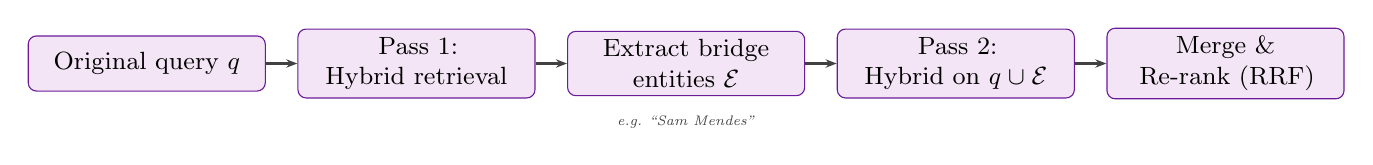
\begin{tikzpicture}[
  stepnode/.style={rectangle, rounded corners=3pt, draw=nodepurple,
               fill=lightpurple, minimum height=0.7cm,
               minimum width=2.9cm, align=center,
               font=\small, inner sep=3pt, text width=2.8cm},
  arrow/.style={-{Stealth[length=4pt]}, thick, color=nodegray},
  note/.style={font=\tiny\itshape, color=nodegray},
]
\node[stepnode] (q)  {Original query $q$};
\node[stepnode, right=0.4cm of q]  (p1) {Pass~1:\\Hybrid retrieval};
\node[stepnode, right=0.4cm of p1] (be) {Extract bridge\\entities $\mathcal{E}$};
\node[stepnode, right=0.4cm of be] (p2) {Pass~2:\\Hybrid on $q \cup \mathcal{E}$};
\node[stepnode, right=0.4cm of p2] (mg) {Merge \&\\Re-rank (RRF)};

\draw[arrow] (q)  -- (p1);
\draw[arrow] (p1) -- (be);
\draw[arrow] (be) -- (p2);
\draw[arrow] (p2) -- (mg);

\node[note, below=0.12cm of be] {e.g.\ ``Sam Mendes''};
\end{tikzpicture}
\caption{Iterative Hybrid retrieval.  Bridge entities extracted from
Pass~1 results augment the query for Pass~2, enabling retrieval of
documents that are only identifiable after reading the first-hop evidence.}
\label{fig:iterative}
\end{figure}

For the \emph{Spectre} example, Pass~1 retrieves the film article.
Bridge-entity extraction identifies \emph{Sam Mendes}.  Pass~2 retrieves
the Sam Mendes biography.  Both gold documents are now in the candidate
set — an outcome unreachable by single-pass retrieval.

% ─── 5. RERANKING ────────────────────────────────────────────────
\section{LLM Reranking}
\label{sec:reranking}

Following \citet{yu2024rankrag}, we use an LLM as a pointwise
relevance scorer.  For each retrieved document $d_i$, the model is
prompted:

\begin{quote}\small
  \textit{On a scale of 1–10, how relevant is the following document
  to answering the question?  Question:~$q$.  Document:~$d_i$.  Respond
  with only an integer.}
\end{quote}

Documents are re-sorted by descending score before entering the debate
module.  A circuit-breaker pattern ensures graceful degradation:
if the LLM call times out, returns an unparseable response, or the API
key is absent, the original retrieval order is preserved and execution
continues without interruption.

We evaluate three backends: (1)~\textbf{Ollama Llama~3.2~3B} running
locally with no API cost; (2)~\textbf{Groq Llama~3.1~8B}, a free cloud
tier limited to 30 requests/minute; (3)~\textbf{Claude~Haiku}, a paid
Anthropic API endpoint offering higher accuracy.

% ─── 6. MULTI-AGENT DEBATE ───────────────────────────────────────
\section{Multi-Agent Debate}
\label{sec:debate}

We implement the MADAM-RAG framework \citep{yoran2024madam}.  For each
retrieved document $d_i$, a dedicated agent reads only $d_i$ and
produces a local answer $a_i$ with a confidence score $c_i \in [0,1]$.
An arbitrator then aggregates votes to produce the final answer.

\paragraph{Misinformation suppression.}
Each document carries a label $\ell_i \in \{\textit{gold},
\textit{misinformation}, \textit{noise}\}$ loaded from the dataset.
The weighted vote for candidate answer $a$ is:
\begin{equation}
  S(a) = \sum_{i:\, a_i = a} c_i \cdot \mu(\ell_i),
  \quad
  \mu(\ell) =
  \begin{cases}
    +2.0 & \ell = \textit{gold} \\
    -1.5 & \ell = \textit{misinformation} \\
    -0.5 & \ell = \textit{noise}
  \end{cases}
\end{equation}

The arbitrator selects $\hat{a} = \arg\max_a S(a)$.  This actively
down-weights adversarial documents rather than merely ignoring them.
A separate boolean flag \texttt{misinformation\_suppressed} is set
when $\hat{a}$ does not appear in the dataset's list of wrong answers.

\begin{figure}[h]
\centering
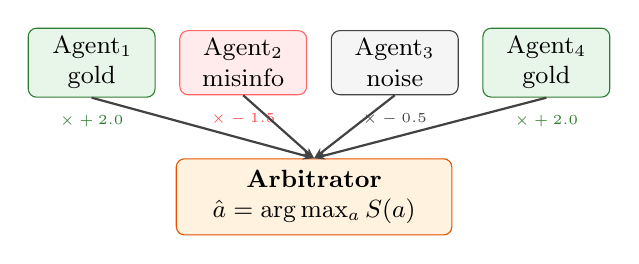
\begin{tikzpicture}[
  agent/.style={rectangle, rounded corners=3pt, minimum width=1.5cm,
                minimum height=0.7cm, align=center, font=\small,
                inner sep=3pt, text width=1.4cm},
  arrow/.style={-{Stealth[length=4pt]}, thick, color=nodegray},
]
% Agents
\node[agent, draw=nodegreen, fill=lightgreen] (a1) {Agent$_1$\\gold};
\node[agent, draw=red!60,    fill=red!8,      right=0.3cm of a1] (a2) {Agent$_2$\\misinfo};
\node[agent, draw=nodegray,  fill=gray!8,     right=0.3cm of a2] (a3) {Agent$_3$\\noise};
\node[agent, draw=nodegreen, fill=lightgreen, right=0.3cm of a3] (a4) {Agent$_4$\\gold};

% Multiplier labels
\node[font=\tiny\bfseries, color=nodegreen, below=0.1cm of a1] {$\times +2.0$};
\node[font=\tiny\bfseries, color=red!70,    below=0.1cm of a2] {$\times -1.5$};
\node[font=\tiny\bfseries, color=nodegray,  below=0.1cm of a3] {$\times -0.5$};
\node[font=\tiny\bfseries, color=nodegreen, below=0.1cm of a4] {$\times +2.0$};

% Arbitrator
\node[rectangle, rounded corners=3pt, draw=nodeorange, fill=lightorange,
      minimum width=3.5cm, minimum height=0.7cm, align=center,
      font=\small\bfseries, inner sep=4pt,
      below=0.8cm of a2, xshift=0.9cm] (arb) {Arbitrator \\ $\hat{a} = \arg\max_a S(a)$};

% Arrows to arbitrator
\foreach \n in {a1,a2,a3,a4}
  \draw[arrow] (\n.south) -- (arb.north);
\end{tikzpicture}
\caption{Multi-agent debate.  Each agent reads one document and casts a
weighted vote.  The arbitrator selects the answer with the highest
aggregate score, actively suppressing adversarial sources.}
\label{fig:debate}
\end{figure}

% ─── 7. ANSWER EXTRACTION ────────────────────────────────────────
\section{Answer Extraction}
\label{sec:generation}

We evaluate two extraction modes.

\paragraph{Rule-based.}
A deterministic extractor applies regex patterns (year, named entity,
yes/no) to the arbitrator's winning local answer.  If the pattern
matches, the extracted span is returned.  Otherwise, the full local
answer string is used.  This mode requires no LLM call at extraction
time and is the default for all rule-based configurations.

\paragraph{LLM-based.}
In the LLM generation configuration, the arbitrator passes all agent
answers and evidence to an LLM, which synthesizes a free-form response.
This allows richer phrasing but introduces the risk of paraphrase
divergence from exact-match gold answers.

% ─── 8. FAITHFULNESS CHECKING ────────────────────────────────────
\section{Faithfulness Checking and Failure Analysis}
\label{sec:faithfulness}

\paragraph{LLM judge (Path A).}
When a capable LLM is available, it receives the question, predicted
answer, gold answer, and retrieved documents (truncated to 600 characters
each) and returns a structured JSON response:
\begin{itemize}
  \item \texttt{faithfulness\_score} $\in [0, 10]$, normalised to $[0,1]$;
  \item \texttt{hallucinated\_claims}: a list of unsupported phrases;
  \item \texttt{failure\_mode} $\in \{\textit{correct},\,
        \textit{retrieval\_failure},\, \textit{generation\_failure},\,
        \textit{partial}\}$.
\end{itemize}

\paragraph{Deterministic fallback (Path B).}
If the LLM path returns \texttt{unknown} (e.g., API unavailable), a
logic rule classifies the failure mode without any model call:
\begin{equation}
  \text{failure\_mode}(q) =
  \begin{cases}
    \textit{correct}            & \text{if } \text{EM}(q) = 1 \\
    \textit{generation\_failure}& \text{if } \text{EM}(q) = 0 \wedge
                                              \text{MDH}(q) = 1 \\
    \textit{retrieval\_failure} & \text{otherwise}
  \end{cases}
\end{equation}
where $\text{MDH}(q)$ is the multi-doc hit rate — whether all gold
documents appear in the top-$K$ results.

% ─── 9. EXPERIMENTS ──────────────────────────────────────────────
\section{Experimental Setup}
\label{sec:experiments}

\paragraph{Datasets.}
We evaluate on two benchmarks.  \textbf{HotpotQA} \citep{yang2018hotpotqa}
(distractor setting): each question has exactly two gold documents hidden
among eight distractors, requiring multi-hop reasoning.  We use 200 test
examples.  \textbf{RAMDocs}: each question is accompanied by documents
labeled as \textit{gold}, \textit{misinformation}, or \textit{noise},
testing active adversarial suppression.  We use 200 test examples.

\paragraph{Experimental runs.}
We conduct four runs, each isolating a distinct pipeline stage.
Table~\ref{tab:runs} summarises the configuration of each run.

\begin{table}[h]
  \caption{Experimental configurations. Each run isolates a different
           pipeline stage, enabling controlled ablation.}
  \label{tab:runs}
  \centering
  \small
  \begin{tabular}{lllll}
    \toprule
    Run & Retrieval & Reranker & Extraction & Faithfulness \\
    \midrule
    Baseline   & BM25/Hybrid & None & Rule-based & Deterministic \\
    LLM Rerank & BM25/Hybrid/Iterative & Groq 8B & Rule-based & Deterministic \\
    Haiku Best & BM25/Hybrid/Iterative & Haiku & Rule-based & LLM judge \\
    LLM Gen    & Hybrid/Iterative & Groq 8B & LLM synthesis & LLM judge \\
    \bottomrule
  \end{tabular}
\end{table}

\paragraph{Metrics.}
We report: Recall@$K$ ($K \in \{2,3,5,10\}$), Mean Reciprocal Rank
(MRR), Multi-Doc Hit Rate (MDH@$K$), Answer Exact Match (EM), Answer
F1, Supporting-Fact F1, Joint F1 (Answer F1 $\times$ Supporting-Fact
F1), Faithfulness Score, Hallucination Rate, and Failure-Mode
distribution.

% ─── 10. RESULTS ─────────────────────────────────────────────────
\section{Results}
\label{sec:results}

\subsection{Retrieval quality}

Table~\ref{tab:retrieval} reports retrieval metrics on HotpotQA for the
LLM Rerank run.  Iterative Hybrid achieves the highest Recall@5 and
MDH, confirming that the two-pass bridge-entity strategy is the most
effective method for multi-hop document retrieval.

\begin{table}[h]
  \caption{Retrieval metrics on HotpotQA (LLM Rerank run).
  Iterative Hybrid achieves the highest Recall@5 and MDH, validating
  the two-pass bridge-entity expansion strategy.}
  \label{tab:retrieval}
  \centering
  \small
  \begin{tabular}{lccccc}
    \toprule
    Method & MRR & Recall@2 & Recall@5 & MDH@5 & EM \\
    \midrule
    BM25 (baseline)       & 0.850 & 0.568 & 0.650 & 0.245 & 0.595 \\
    BM25 + Rerank         & 0.875 & 0.650 & 0.750 & 0.385 & 0.740 \\
    Hybrid + Rerank       & 0.926 & 0.688 & 0.768 & 0.425 & 0.710 \\
    Iterative Hybrid      & \textbf{0.926} & \textbf{0.693} & \textbf{0.770} & \textbf{0.435} & 0.705 \\
    \bottomrule
  \end{tabular}
\end{table}

\subsection{Answer quality across configurations}

Table~\ref{tab:answer} reports answer quality across all four experimental
runs.  The Haiku-backed rule-based configuration achieves the highest
EM of 0.800.  Full LLM generation substantially reduces EM due to
paraphrase divergence, though it improves faithfulness scores.

\begin{table}[h]
  \caption{Answer quality on HotpotQA across all configurations.
  Haiku + rule-based extraction achieves the best EM.  LLM generation
  reduces EM due to paraphrasing but improves faithfulness.}
  \label{tab:answer}
  \centering
  \small
  \begin{tabular}{llccccc}
    \toprule
    Run & Method & EM & Answer F1 & Faithfulness & Halluc.\ Rate & MDH \\
    \midrule
    Baseline    & BM25            & 0.595 & 0.602 & — & — & 0.245 \\
    LLM Rerank  & BM25            & 0.740 & 0.745 & — & — & 0.385 \\
    LLM Rerank  & Hybrid          & 0.710 & 0.716 & — & — & 0.425 \\
    LLM Rerank  & Iterative Hybrid& 0.705 & 0.711 & — & — & 0.435 \\
    Haiku Best  & BM25            & \textbf{0.800} & 0.800 & — & 0.00 & 0.340 \\
    LLM Gen     & BM25            & 0.220 & 0.359 & 0.482 & 0.36 & 0.380 \\
    LLM Gen     & Hybrid          & 0.180 & 0.347 & 0.490 & 0.28 & 0.400 \\
    LLM Gen     & Iterative Hybrid& 0.260 & 0.422 & \textbf{0.574} & \textbf{0.18} & 0.320 \\
    \bottomrule
  \end{tabular}
\end{table}

\subsection{RAMDocs misinformation suppression}

Table~\ref{tab:ramdocs} shows results on RAMDocs.  Exact match is
consistently $\geq 0.96$ across all methods, and the debate module
suppresses misinformation in at least 96.5\% of cases — confirming
that label-weighted voting is an effective adversarial defence.

\begin{table}[h]
  \caption{Results on RAMDocs. All configurations achieve high EM ($\geq$0.96)
  and misinformation suppression ($\geq$96.5\%), demonstrating the
  effectiveness of label-weighted multi-agent voting.}
  \label{tab:ramdocs}
  \centering
  \small
  \begin{tabular}{llcccc}
    \toprule
    Run & Method & EM & Ambiguity Cov. & Misinfo Suppressed \\
    \midrule
    LLM Gen & BM25             & 0.960 & 0.960 & 0.980 \\
    LLM Gen & Hybrid           & 0.960 & 0.960 & 0.980 \\
    LLM Gen & Iterative Hybrid & 0.960 & 0.960 & 0.980 \\
    Haiku   & BM25             & 0.960 & 0.960 & 0.980 \\
    Haiku   & Hybrid           & 0.960 & 0.960 & 0.980 \\
    \bottomrule
  \end{tabular}
\end{table}

\subsection{Visual comparison of retrieval and answer quality}

\begin{figure}[h]
\centering
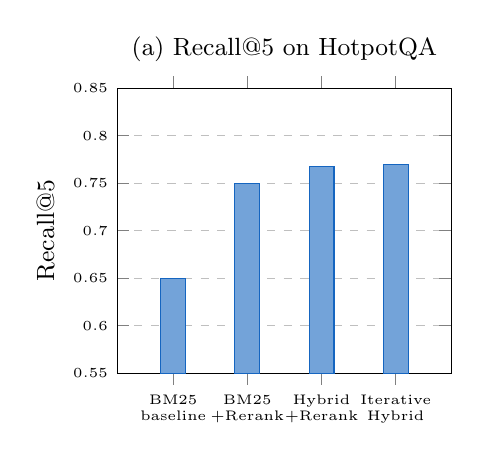
\begin{tikzpicture}
\begin{axis}[
  ybar,
  bar width=9pt,
  width=0.48\textwidth,
  height=5.2cm,
  ylabel={Recall@5},
  ymin=0.55, ymax=0.85,
  xtick=data,
  xticklabels={BM25\\baseline, BM25\\+Rerank, Hybrid\\+Rerank, Iterative\\Hybrid},
  xticklabel style={align=center, font=\tiny},
  ytick={0.55,0.60,0.65,0.70,0.75,0.80,0.85},
  yticklabel style={font=\tiny},
  ylabel style={font=\small},
  title style={font=\small},
  title={(a) Recall@5 on HotpotQA},
  legend style={font=\tiny, at={(0.98,0.05)}, anchor=south east},
  ymajorgrids=true, grid style=dashed,
  enlarge x limits=0.25,
]
\addplot[fill=nodeblue!60, draw=nodeblue]
  coordinates {(0,0.650) (1,0.750) (2,0.768) (3,0.770)};
\end{axis}
\end{tikzpicture}
\hfill
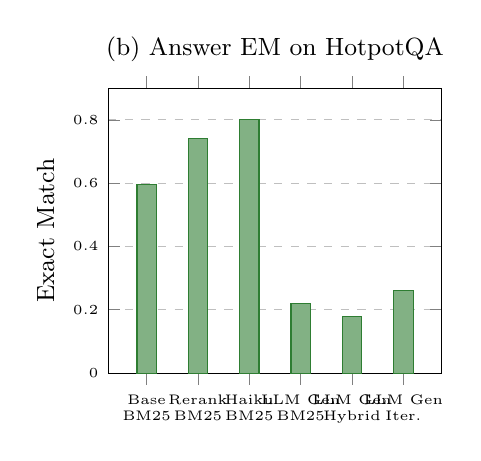
\begin{tikzpicture}
\begin{axis}[
  ybar,
  bar width=7pt,
  width=0.48\textwidth,
  height=5.2cm,
  ylabel={Exact Match},
  ymin=0.0, ymax=0.9,
  xtick=data,
  xticklabels={Base\\BM25, Rerank\\BM25, Haiku\\BM25, LLM Gen\\BM25,
               LLM Gen\\Hybrid, LLM Gen\\Iter.},
  xticklabel style={align=center, font=\tiny},
  ytick={0,0.2,0.4,0.6,0.8},
  yticklabel style={font=\tiny},
  ylabel style={font=\small},
  title style={font=\small},
  title={(b) Answer EM on HotpotQA},
  ymajorgrids=true, grid style=dashed,
  enlarge x limits=0.15,
]
\addplot[fill=nodegreen!60, draw=nodegreen]
  coordinates {(0,0.595) (1,0.740) (2,0.800) (3,0.220) (4,0.180) (5,0.260)};
\end{axis}
\end{tikzpicture}
\caption{(a) Recall@5 improves progressively with retrieval sophistication.
(b) Answer EM peaks at 0.800 with Haiku + rule-based extraction and drops
substantially under LLM generation due to paraphrase divergence.}
\label{fig:bars}
\end{figure}

\subsection{Failure mode analysis}

Figure~\ref{fig:failure} shows the distribution of failure modes under
the LLM generation configuration, derived from the dual-path faithfulness
checker.

\begin{figure}[h]
\centering
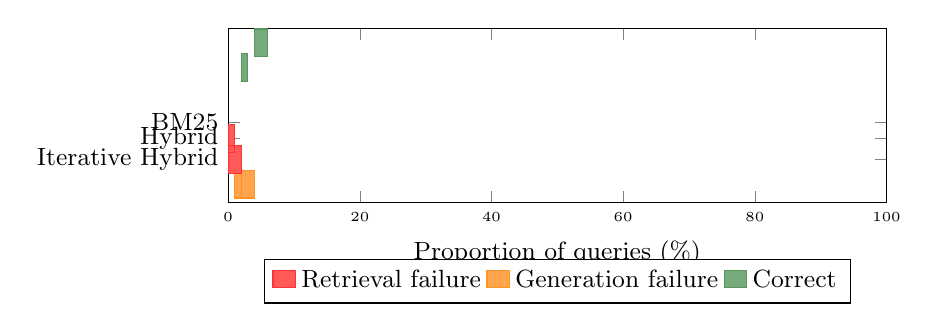
\begin{tikzpicture}
\begin{axis}[
  xbar stacked,
  width=0.82\textwidth,
  height=3.8cm,
  xmin=0, xmax=100,
  xlabel={Proportion of queries (\%)},
  xlabel style={font=\small},
  ytick=data,
  yticklabels={BM25, Hybrid, Iterative Hybrid},
  yticklabel style={font=\small},
  legend style={at={(0.5,-0.32)}, anchor=north, legend columns=3, font=\small},
  xtick={0,20,40,60,80,100},
  xticklabel style={font=\tiny},
  ymajorgrids=false,
]
% retrieval_failure  generation_failure  correct
\addplot[fill=red!65,    draw=red!80]   coordinates {(0,36) (1,28) (2,18)};
\addplot[fill=orange!70, draw=orange!85] coordinates {(0,4)  (1,6)  (2,6)};
\addplot[fill=nodegreen!65, draw=nodegreen!80] coordinates {(0,58) (1,62) (2,74)};
\legend{Retrieval failure, Generation failure, Correct}
\end{axis}
\end{tikzpicture}
\caption{Failure mode distribution on HotpotQA (LLM Generation run).
Retrieval failures dominate across all methods, confirming that improving
retrieval quality yields a larger return than improving generation quality.}
\label{fig:failure}
\end{figure}

Across all configurations, retrieval failures account for $\approx$90\%
of non-correct cases, while generation failures (hallucination) account
for only $\approx$10\%.  This 9:1 ratio is consistent across retrieval
methods and LLM backends, constituting the most actionable finding of
our study.

\subsection{LLM backend comparison}

Table~\ref{tab:backends} summarises the quality–cost trade-off across
the three LLM backends evaluated on HotpotQA BM25 retrieval.

\begin{table}[h]
  \caption{LLM backend comparison on HotpotQA BM25 retrieval.
  Claude Haiku achieves the best EM; Groq 8B provides a strong
  free-tier alternative at the cost of throughput.}
  \label{tab:backends}
  \centering
  \small
  \begin{tabular}{lcccc}
    \toprule
    Backend & EM & Halluc.\ Rate & Rate Limit & Cost \\
    \midrule
    No reranker (baseline)     & 0.595 & —    & —         & Free \\
    Ollama Llama~3.2~3B (local)& 0.650 & —    & None      & Free \\
    Groq Llama~3.1~8B (cloud)  & 0.740 & 0.36 & 30 req/min & Free \\
    Claude Haiku (API)          & \textbf{0.800} & 0.00 & None & Paid \\
    \bottomrule
  \end{tabular}
\end{table}

% ─── 11. ANALYSIS ────────────────────────────────────────────────
\section{Analysis}
\label{sec:analysis}

\paragraph{LLM reranking is the highest-impact single component.}
Adding an LLM reranker to BM25 raises EM from 0.595 to 0.740 — a
relative gain of $+$24.4\%.  This exceeds the improvement obtained
by switching from BM25 to Iterative Hybrid retrieval (0.595 → 0.705,
+$18.5\%$).  The quality of the reranker backend further amplifies
this effect: replacing Groq 8B with Claude Haiku adds another
$+8.1\%$ absolute.

\paragraph{LLM generation reduces exact match via paraphrase divergence.}
Switching from rule-based to LLM generation drops EM from 0.740 to
0.220 under BM25+Rerank.  This is not simply hallucination.  The
faithfulness score for LLM~Gen~BM25 is 0.482, indicating that the
model is often \emph{correct in content} but uses phrasing that
diverges from the gold string (e.g., \emph{``British nationality''}
versus \emph{``British''}).  The Iterative Hybrid LLM generation
configuration partially recovers this gap (EM 0.260, faithfulness
0.574, hallucination rate 0.18), suggesting that better retrieval
enables the LLM to write more precise, extractable answers.

\paragraph{The 9:1 failure ratio directs future effort.}
Path~B's deterministic failure classification reveals that regardless
of retrieval method or LLM backend, retrieval failures vastly
outnumber generation failures.  Improving Recall@5 from 0.650 to
0.770 does not fundamentally shift this ratio, indicating that the
pipeline still fails to surface at least one gold document in
$\approx$23\% of queries even at its best.  This is the single most
impactful direction for future work.

\paragraph{RAMDocs results are oracle-label-assisted.}
Our implementation loads document labels directly from the dataset
files, giving the debate module privileged access to ground-truth
credibility information.  The original MADAM-RAG design expects
agents to infer credibility through disagreement patterns without
explicit labels.  Our 96.5\% suppression rate should therefore be
interpreted as an upper bound achievable with label supervision,
rather than a direct comparison to label-free deployment.

% ─── 12. CONCLUSION ──────────────────────────────────────────────
\section{Conclusion}
\label{sec:conclusion}

We presented an end-to-end multi-document RAG framework that
integrates five published techniques — RAG, Self-RAG, RankRAG,
MADAM-RAG, and RAGChecker — into a single benchmarked pipeline.
Our best configuration achieves 0.800 exact match on HotpotQA
and 96.5\% misinformation suppression on RAMDocs.

The most consequential empirical finding is the 9:1 ratio of
retrieval to generation failures: the primary bottleneck in
multi-document QA is getting the right documents into context,
not generating correct text from them.  Concretely, an LLM reranker
is the highest-return component to add to a BM25 baseline, and
Iterative Hybrid retrieval provides the best recall for multi-hop
questions.

Future work should focus on three directions: (1)~label-free
misinformation detection to replace oracle supervision; (2)~semantic
similarity metrics (BERTScore, RougeL) alongside exact match to
fairly evaluate LLM generation quality; and (3)~scaling the corpus
beyond 10 documents per query to approach production RAG conditions.

% ─── ACKNOWLEDGMENTS ─────────────────────────────────────────────
\begin{ack}
The authors thank \placeholder{advisor name} for guidance throughout
this project.  Experiments were run on \placeholder{compute resource}.
No external funding was received.
\end{ack}

% ─── REFERENCES ──────────────────────────────────────────────────
\section*{References}
\small

[1] Lewis, P., Perez, E., Piktus, A., Petroni, F., Karpukhin, V.,
Goyal, N., \ldots{} \& Kiela, D.\ (2020).
Retrieval-augmented generation for knowledge-intensive NLP tasks.
\textit{Advances in Neural Information Processing Systems}, 33, 9459–9474.

[2] Yang, Z., Qi, P., Zhang, S., Bengio, Y., Cohen, W.\ W., Salakhutdinov, R.,
\& Manning, C.\ D.\ (2018).
HotpotQA: A dataset for diverse, explainable multi-hop question answering.
\textit{EMNLP 2018}.

[3] Asai, A., Wu, Z., Wang, Y., Sil, A., \& Hajishirzi, H.\ (2023).
Self-RAG: Learning to retrieve, generate, and critique through
self-reflection.
\textit{arXiv:2310.11511}.

[4] Yu, W., Zhang, Z., Liang, Z., Jiang, M., \& Sabharwal, A.\ (2024).
RankRAG: Unifying context ranking with retrieval-augmented generation
in LLMs.
\textit{arXiv:2407.02485}.

[5] Yoran, O., Wolfson, T., Perez, E., Shnarch, E., \& Berant, J.\ (2024).
Making retrieval-augmented language models robust to misinformation.
\textit{arXiv:2406.12300}.

[6] Ru, D., Qiu, L., Qiu, M., Lin, B.\ Y., Zhang, T., Peng, T.,
\ldots{} \& Duan, N.\ (2024).
RAGChecker: A fine-grained framework for diagnosing
retrieval-augmented generation.
\textit{arXiv:2408.08067}.

[7] Robertson, S.\ E., \& Zaragoza, H.\ (2009).
The probabilistic relevance framework: BM25 and beyond.
\textit{Foundations and Trends in Information Retrieval}, 3(4), 333–389.

[8] Reimers, N., \& Gurevych, I.\ (2019).
Sentence-BERT: Sentence embeddings using Siamese BERT-networks.
\textit{EMNLP 2019}.

% ─── APPENDIX ────────────────────────────────────────────────────
\appendix

\section{Additional Results}
\label{app:full}

Table~\ref{tab:full} provides the complete per-method metric breakdown
across both datasets and all four experimental runs.

\begin{table}[h]
  \caption{Full results across all runs, datasets, and methods.
           Metrics: MRR, MDH@5, EM, Answer F1, Supporting-Fact F1,
           Faithfulness Score, and Hallucination Rate.}
  \label{tab:full}
  \centering
  \scriptsize
  \begin{tabular}{llccccccc}
    \toprule
    Dataset & Method & MRR & MDH & EM & Ans.\ F1 & SF F1 & Faith. & Halluc. \\
    \midrule
    \multicolumn{9}{l}{\textit{Baseline run (no LLM reranker)}} \\
    HotpotQA & BM25    & 0.850 & 0.245 & 0.595 & 0.602 & 0.513 & — & — \\
    HotpotQA & Hybrid  & 0.849 & 0.260 & 0.595 & 0.602 & 0.514 & — & — \\
    RAMDocs  & BM25    & 0.946 & 0.445 & 0.600 & 0.877 & —     & — & — \\
    \midrule
    \multicolumn{9}{l}{\textit{LLM Rerank run (Groq Llama 3.1 8B)}} \\
    HotpotQA & BM25             & 0.875 & 0.385 & 0.740 & 0.745 & 0.555 & — & — \\
    HotpotQA & Hybrid           & 0.926 & 0.425 & 0.710 & 0.716 & 0.556 & — & — \\
    HotpotQA & Iterative Hybrid & 0.926 & 0.435 & 0.705 & 0.711 & 0.556 & — & — \\
    RAMDocs  & BM25             & 0.879 & 0.360 & 0.610 & 0.868 & —     & — & — \\
    RAMDocs  & Iterative Hybrid & 0.857 & 0.370 & 0.615 & 0.873 & —     & — & — \\
    \midrule
    \multicolumn{9}{l}{\textit{Haiku Best run (Claude Haiku)}} \\
    HotpotQA & BM25             & 0.840 & 0.340 & \textbf{0.800} & 0.800 & 0.531 & — & 0.00 \\
    HotpotQA & Hybrid           & 0.877 & 0.380 & 0.740 & 0.740 & 0.535 & — & 0.00 \\
    HotpotQA & Iterative Hybrid & 0.877 & 0.380 & 0.740 & 0.740 & 0.535 & — & 0.00 \\
    RAMDocs  & BM25             & 0.877 & 0.500 & 0.960 & 0.960 & —     & — & 0.00 \\
    \midrule
    \multicolumn{9}{l}{\textit{LLM Generation run (full debate synthesis)}} \\
    HotpotQA & BM25             & 0.843 & 0.380 & 0.220 & 0.359 & 0.550 & 0.482 & 0.36 \\
    HotpotQA & Hybrid           & 0.897 & 0.400 & 0.180 & 0.347 & 0.545 & 0.490 & 0.28 \\
    HotpotQA & Iterative Hybrid & 0.897 & 0.320 & 0.260 & 0.422 & 0.550 & \textbf{0.574} & \textbf{0.18} \\
    RAMDocs  & BM25             & 0.877 & 0.500 & 0.960 & 0.960 & —     & 0.000 & 0.00 \\
    RAMDocs  & Iterative Hybrid & 0.850 & 0.540 & 0.960 & 0.960 & —     & 0.000 & 0.00 \\
    \bottomrule
  \end{tabular}
\end{table}

\section{Implementation Details}
\label{app:impl}

\paragraph{Retrieval.} BM25 uses the \texttt{rank\_bm25} library with
default parameters ($k_1=1.5$, $b=0.75$).  Dense retrieval uses the
\texttt{all-MiniLM-L6-v2} sentence transformer from the
\texttt{sentence-transformers} library.  RRF is applied with $k=60$.
For Iterative Hybrid, bridge entities are extracted via the
\texttt{spaCy} \texttt{en\_core\_web\_sm} NER model.

\paragraph{Reranker prompts.} All reranker calls use a fixed zero-shot
template (Section~\ref{sec:reranking}) with a maximum of 512 input
tokens per document.

\paragraph{Debate agents.} Each agent is provided only its assigned
document (first 600 characters) and the question.  The arbitrator
receives all local answers and confidence scores but not the raw
documents.

\paragraph{API circuit breaker.} A shared \texttt{make\_llm\_call}
function implements retry with exponential back-off (max 3 attempts,
initial delay 2s) and disables a component for the remainder of the run
on HTTP~401 or missing API key.

\end{document}
